\chapter{Opis projektnog zadatka}
		
		U velikoj konkurenciji različitih pub kvizova kojoj i sami svjedočimo, želja je svakog sastavljača privući što veći broj ekipa i učiniti kviz što je moguće zanimljivijim. Svaki pojedini igrač ili tim želi pronaći pub kviz na kojem mu najbolje odgovara koncept pitanja i gdje je atmosfera jednostavno priča za sebe. Kako bi se povezali sastavljači, kvizaši, ali i oni koji to tek žele postati ili jednostavno probati nešto novo, cilj je razviti aplikaciju koja će znatno olakšati taj proces i ponuditi dodatne funkcionalnosti.
		\newline \newline
		Glavni je cilj ove aplikacije omogućiti sastavljačima kvizova objavu nadolazećih pub kvizova koje organiziraju i osigurati igračima da vide koliko se raznolikih kvizova održava u njihovoj blizini, kao i kada se održavaju oni za koje su najviše zainteresirani. S obzirom na to da često postoje osobe koje žele igrati neki pub kviz, ali nažalost nemaju ekipu, aplikacija će riješiti i taj problem. Igrač koji nema ekipu, a ipak želi sudjelovati na pub kvizu, moći će u aplikaciji pronaći tim kojemu bi najviše odgovarao kao suigrač i tako zaigrati kviz.
		\newline \newline
		\underbar{Neregistrirani korisnik} imat će mogućnost isključivo pregleda pub kvizova, ali s ograničenim uvidom u detalje objavljenih događaja. Moći će vidjeti naziv kviza, ime kafića, vrijeme održavanja te vrstu kviza, ali za sve ostale pojedinosti prvo se mora registrirati u sustav.
		\newline \newline
		\underbar{Registrirani korisnik} može biti ili sastavljač ili igrač kviza. Svaka od ovih uloga ima drugačiji skup mogućnosti u aplikaciji. Iznimno, ako je jedan korisnik sastavljač pub kvizova, ali isto tako i sudjeluje na nekim drugima kao igrač, on može imati obje uloge u aplikaciji. Prilikom registracije korisnik najprije odabire ulogu na temelju koje ispunjava prilagođenu formu. Ako se registrira kao igrač ili istovremeno kao igrač i sastavljač onda unosi sljedeće podatke:
		\begin{packed_item}
			\item \textit{\textbf{Ime}}
			\item \textit{\textbf{Prezime}}
			\item \textit{\textbf{Nadimak}}
			\item \textit{\textbf{Email adresa}}
			\item \textit{\textbf{Lozinka}}
			\item \textit{\textbf{Područja znanja za kviz}}
            \item \textit{\textbf{Imaš ekipu?}}
            \item[] \begin{packed_item}
            	\item {[DA]  \textbf{ Naziv ekipe}}
            	\item {[NE]}
           		    \end{packed_item}
            \item \textit{Slika}
           	\item \textit{Broj telefona}
            
		\end{packed_item}
		
		\textit{Pri čemu su podebljani podaci obvezni za unijeti.} Ako ipak odabere samo ulogu sastavljača, onda unosi ove podatke:
		\begin{packed_item}
			\item \textit{\textbf{Ime}}
			\item \textit{\textbf{Prezime}}
			\item \textit{\textbf{Nadimak}}
			\item \textit{\textbf{Email adresa}}
			\item \textit{\textbf{Lozinka}}
			\item \textit{Slika}
			\item \textit{Broj telefona}
			
		\end{packed_item}
	
		U slučaju da korisnik ima svoju pub kviz ekipu, pri registraciji će odabrati vrijednost DA za polje Imaš ekipu? te će morati obvezno unijeti naziv svoje ekipe. Inače, ako nema ekipu odabrat će opciju NE.
		\newline \newline
		\underbar{Sastavljač pub kvizova}, ujedno je i organizator događaja (pub kviza) te kroz aplikaciju ima mogućnost objaviti nadolazeći događaj tako da prilikom objave unese sve potrebne podatke bitne za kviz:
		\begin{packed_item}
			\item \textit{\textbf{Naziv kviza}}
			\item \textit{\textbf{Kratki opis}}
			\item \textit{\textbf{Ime kafića}}
			\item \textit{\textbf{Vrijeme održavanja}}
			\item \textit{\textbf{Lokacija}}
			\item \textit{\textbf{Maksimalan broj ekipa}}
			\item \textit{\textbf{Iznos kotizacije}}
			\item \textit{\textbf{Nazivi nagrada}}
			\item \textit{\textbf{Vrsta kviza}}
			\item \textit{\textbf{Informacije o sastavljaču}}
			
		\end{packed_item}
	
		Pri kreiranju nove objave događaja potrebno je paziti da sastavljač ne smije objaviti više događaja koji su u isto vrijeme (s preklapanjem termina). Ako korisnik sastavljač ima i ulogu igrača, treba dodatno paziti da u isto vrijeme događaja koji je korisnik objavio, isti korisnik nije prijavljen kao igrač na neki od kvizova. Sastavljač može vidjeti sve objave pub kvizova u aplikaciji na pregledu "Svi pub kvizovi", a svoje objave vidi na pregledu "Moji pub kvizovi". Uz to, sastavljač može pregledati i uređivati svoj profil na pregledu "Moj profil" s podacima unesenim pri registraciji.
		\newline \newline
		\underbar{Igrač pub kvizova} ima dvije glavne mogućnosti u aplikaciji, a to su pronalazak ekipe (samo za one igrače koji ju nemaju) i prijava svoje ekipe na neki od objavljenih kvizova. Ako pri registraciji korisnik navede da nema vlastitu ekipu, onda u aplikaciji ima mogućnost pronaći ju tako da odabere opciju „Pronađi tim“ i aplikacija će ga spojiti s ekipom kojoj najviše odgovara (većina područja znanja u kojima je dobar nedostaju ekipi s kojom će ga aplikacija spojiti). Kada je korisniku pronađen tim, dolazi mu obavijest s nazivom ekipe i brojem članova. Također, svakom igraču te ekipe dolazi obavijest da su dobili novog igrača i popis njegovih boljih područja znanja s kojima će doprinijeti timu. Igrači koji imaju svoju ekipu mogu je napustiti odabirom opcije "Napusti tim". Igrač može vidjeti sve objave pub kvizova u aplikaciji na pregledu "Svi pub kvizovi", a događaje na koje je prijavljen može vidjeti na pregledu "Moji pub kvizovi". Također, igrači mogu prijaviti svoju ekipu na kviz, tako da 1 igrač iz ekipe prijavljuje cijelu ekipu na određeni kviz. Pri tome treba paziti da jedna ekipa ne bude prijavljena na više različitih kvizova u isto vrijeme. Kada igrač uspješno prijavi svoju ekipu na kviz, njemu i njegovim suigračima dolazi obavijest da su prijavljeni na novi kviz i na objavi za taj događaj broj slobodnih mjesta se ažurira (jedno slobodno mjesto manje). Uz to, igrač može pregledati i uređivati svoj profil na pregledu "Moj profil" s podacima unesenim pri registraciji.
		\newline \newline
		\underbar{Administrator} sustava uz ovlasti svih korisnika ima i neke dodatne mogućnosti u aplikaciji, a to su: blokiranje korisnika koji krše pravila sustava (na primjer imaju nepristojan nadimak ili naziv ekipe), odobravanje ili zabranjivanje objava za pub kvizove koje prethodno kreiraju sastavljači te mogućnost naknadnog brisanja istih događaja. Također, administrator može dodati administratorska prava drugim korisnicima.
		\newline \newline
		Aplikacija za sve prijavljene korisnike  treba omogućiti pretraživanje objavljenih događaja te filtriranje prema određenim parametrima. Funkcionalnost pretraživanja ostvarena je okvirom za pretraživanje (eng. search bar), pomoću kojeg prijavljeni korisnik može pronaći određeni događaj unoseći njegov naziv ili ime kafića u kojem se kviz održava. Filtriranje se dodatno ostvaraju na način da korisnik odabire željene vrijednosti ili raspon vrijednosti za svoju udaljenost od kafića gdje se kviz održava, iznos kotizacije, vrstu kviza ili slično.
		\newline \newline
		Također, svi igrači pub kvizova imaju mogućnost uvida u statističke detalje na pregledu "Statistika", u kojem mogu vidjeti i usporediti  prikazane podatke u obliku grafa ili tablice, a bilježi se prosječan broj ekipa po kvizu za nekog sastavljača, broj održanih kvizova u posljednjih tjedan dana te prosječna popunjenost kviza za pojedinu vrstu kviza.
		\newline \newline
		Pretpostavka je da je 1 igrač fiksno u 1 ekipi te da ekipa ima maksimalno 5 članova.
		\newline \newline
		Ovaj projekt potencijalno bi mogao koristiti za organizaciju i prijave na sve postojeće pub kvizove u Hrvatskoj, a posebna prednost je što bi sve objave kvizova bile razvrstane, pregledne i skupljene na jednom mjestu kako bi korisnici mogli brzo i jednostavno dobiti bitne informacije o pojedinom događaju. 
		Zainteresirani skup korisnika činili bi svi sastavljači i organizatori kvizova, članovi ekipa te igrači koji žele ići na neki kviz, ali još nemaju suigrače. 
		Opseg projektnog zadatka ponajprije obuhvaća funkcionalnosti objave kvizova, prijave i pronalazak ekipe, a moguće je i dobiti dodatne informacije o pojedinom kvizu ili sastavljaču. 
		Također, projektni zadatak mogao bi se nadograditi tako da sastavljači mogu dodati slike, poredak ekipa i nekoliko pitanja sa svojih bivših događaja te se na taj način predstaviti svim igračima koji pregledavaju njihove profile. Dodatno proširenje bilo bi uvođenje recenzija za kvizove i sastavljače te komentari i osvrti o pojedinim događajima.
		Iako ne postoje programska rješenja koja nude sve mogućnosti kao ova aplikacija, postoje različite web stranice gdje se može pronaći popis kvizova za određeno mjesto i datum te osnovne informacije o kreiranim događajima. Kao jednu od najpopularnijih navodimo \url{https://www.pubquizzers.com/index.php}.
		
		\begin{figure}[H]
			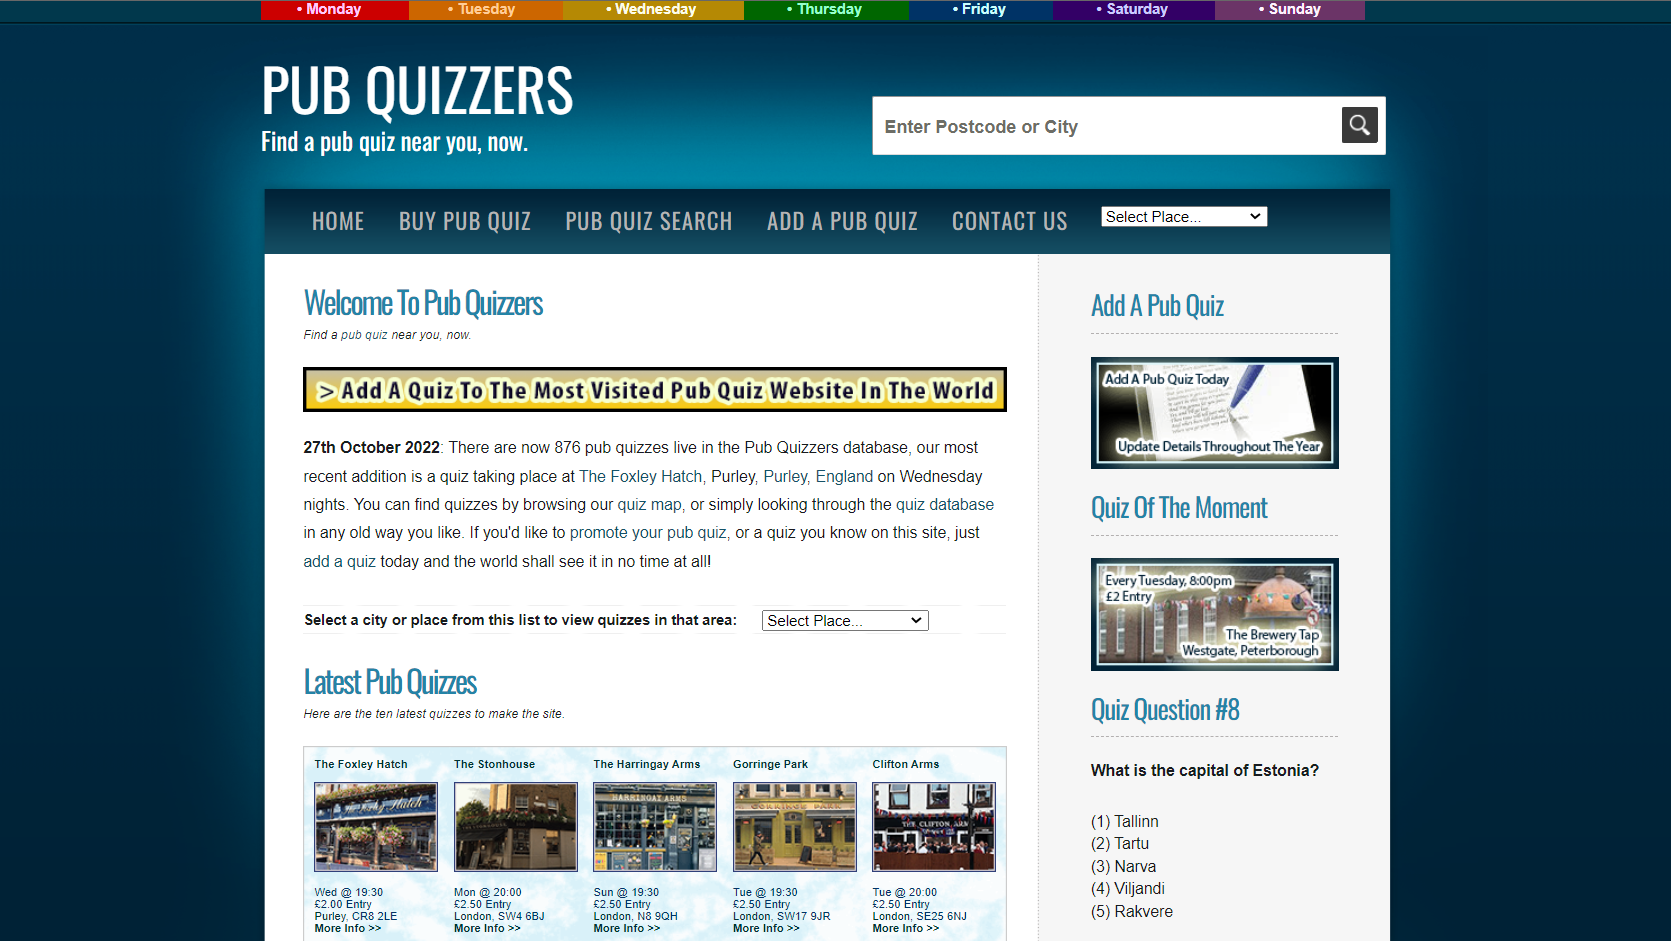
\includegraphics[width=\textwidth]{slike/slicnoRjesenje.PNG} 
			\caption{Primjer sličnog rješenja}
			\label{fig:slicnoRjesenje}
		\end{figure}

		\section{Primjeri u \LaTeX u}
		
		\textit{Ovo potpoglavlje izbrisati.}\\

		U nastavku se nalaze različiti primjeri kako koristiti osnovne funkcionalnosti \LaTeX a koje su potrebne za izradu dokumentacije. Za dodatnu pomoć obratiti se asistentu na projektu ili potražiti upute na sljedećim web sjedištima:
		\begin{itemize}
			\item Upute za izradu diplomskog rada u \LaTeX u - \url{https://www.fer.unizg.hr/_download/repository/LaTeX-upute.pdf}
			\item \LaTeX\ projekt - \url{https://www.latex-project.org/help/}
			\item StackExchange za Tex - \url{https://tex.stackexchange.com/}\\
		
		\end{itemize} 	


		
		\noindent \underbar{podcrtani tekst}, \textbf{podebljani tekst}, 	\textit{nagnuti tekst}\\
		\noindent \normalsize primjer \large primjer \Large primjer \LARGE {primjer} \huge {primjer} \Huge primjer \normalsize
				
		\begin{packed_item}
			
			\item  primjer
			\item  primjer
			\item  primjer
			\item[] \begin{packed_enum}
				\item primjer
				\item[] \begin{packed_enum}
					\item[1.a] primjer
					\item[b] primjer
				\end{packed_enum}
				\item primjer
			\end{packed_enum}
			
		\end{packed_item}
		
		\noindent primjer url-a: \url{https://www.fer.unizg.hr/predmet/proinz/projekt}
		
		\noindent posebni znakovi: \# \$ \% \& \{ \} \_ 
		$|$ $<$ $>$ 
		\^{} 
		\~{} 
		$\backslash$ 
		
		
		\begin{longtblr}[
			label=none,
			entry=none
			]{
				width = \textwidth,
				colspec={|X[8,l]|X[8, l]|X[16, l]|}, 
				rowhead = 1,
			} %definicija širine tablice, širine stupaca, poravnanje i broja redaka naslova tablice
			\hline \textbf{naslov unutar tablice} & \\ \hline[3pt]
			\SetCell{LightGreen}IDKorisnik & INT	&  	Lorem ipsum dolor sit amet, consectetur adipiscing elit, sed do eiusmod  	\\ \hline
			korisnickoIme	& VARCHAR &   	\\ \hline 
			email & VARCHAR &   \\ \hline 
			ime & VARCHAR	&  		\\ \hline 
			\SetCell{LightBlue} primjer	& VARCHAR &   	\\ \hline 
		\end{longtblr}
		

		\begin{longtblr}[
				caption = {Naslov s referencom izvan tablice},
				entry = {Short Caption},
			]{
				width = \textwidth, 
				colspec = {|X[8,l]|X[8,l]|X[16,l]|}, 
				rowhead = 1,
			}
			\hline
			\SetCell{LightGreen}IDKorisnik & INT	&  	Lorem ipsum dolor sit amet, consectetur adipiscing elit, sed do eiusmod  	\\ \hline
			korisnickoIme	& VARCHAR &   	\\ \hline 
			email & VARCHAR &   \\ \hline 
			ime & VARCHAR	&  		\\ \hline 
			\SetCell{LightBlue} primjer	& VARCHAR &   	\\ \hline 
		\end{longtblr}
	


		
		
		%unos slike
		\begin{figure}[H]
			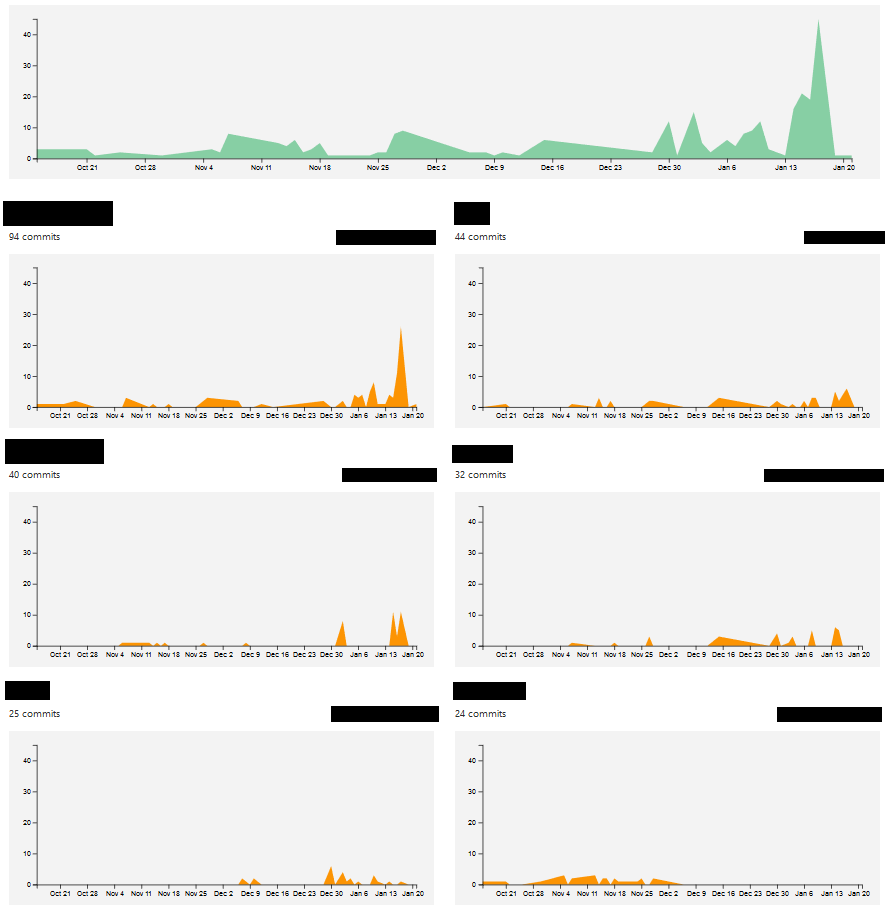
\includegraphics[scale=0.4]{slike/aktivnost.PNG} %veličina slike u odnosu na originalnu datoteku i pozicija slike
			\centering
			\caption{Primjer slike s potpisom}
			\label{fig:promjene}
		\end{figure}
		
		\begin{figure}[H]
			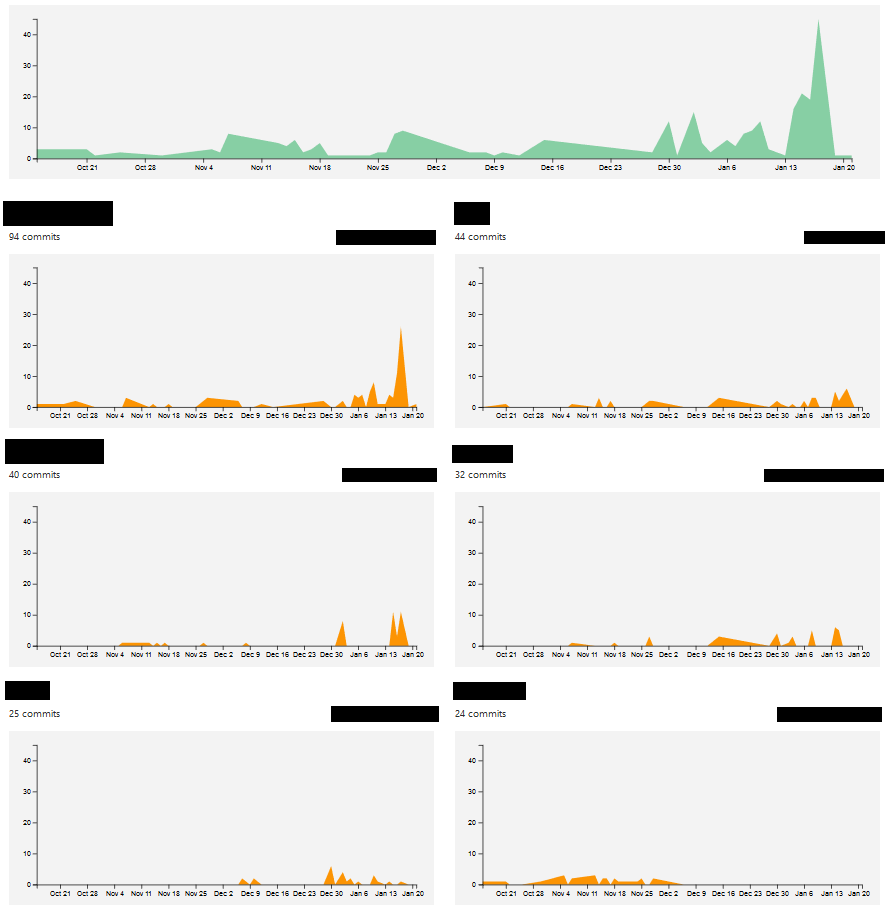
\includegraphics[width=\textwidth]{slike/aktivnost.PNG} %veličina u odnosu na širinu linije
			\caption{Primjer slike s potpisom 2}
			\label{fig:promjene2} %label mora biti drugaciji za svaku sliku
		\end{figure}
		
		Referenciranje slike \ref{fig:promjene2} u tekstu.
		
		\eject
		
	